\chapter{Исследовательская часть}

\section{Технические характеристики}

Технические характеристики устройства, на котором выполнялись замеры по времени:

\begin{itemize}
	\item Процессор: Apple M1 Pro \cite{m1}
	\item Оперативная память: 32 ГБайт.
	\item Операционная система: macOS Ventura 13.5.2. \cite{macOS}
\end{itemize}

При замерах времени ноутбук был включен в сеть электропитания и был нагружен только системными приложениями.

\section{Демонстрация работы программы}

На изображении \ref{img:demonstration} представлена иллюстрация работы разработанного программного продукта. 
Конкретно, демонстрируются результаты выполнения алгоритмов для вычисления произведения двух матриц. 
\clearpage
\begin{figure}[h]
	\centering
	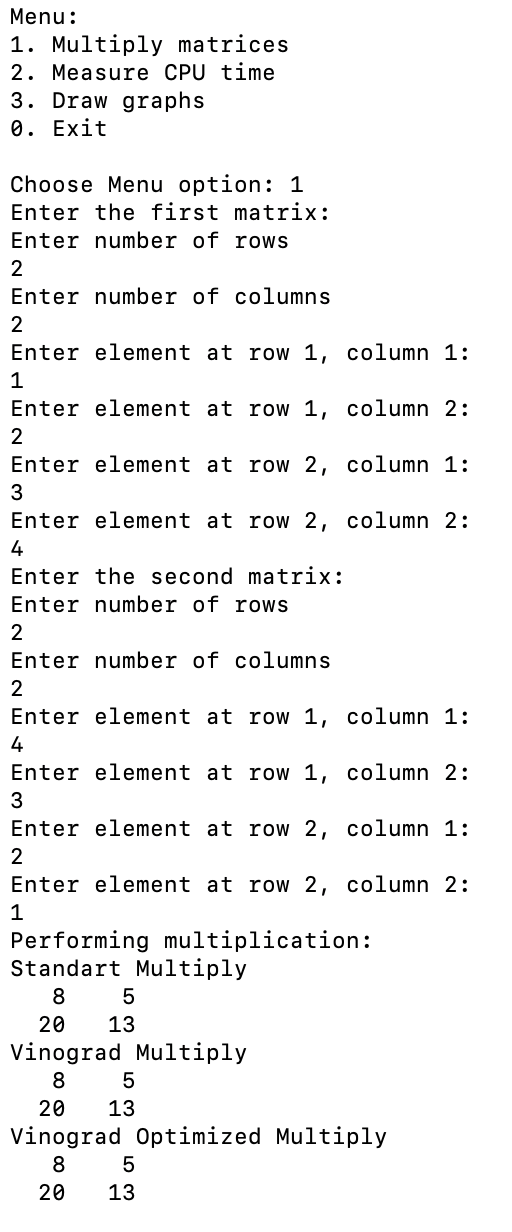
\includegraphics[height=0.7\textheight]{img/example.png}
	\caption{Демонстрация работы программы при вычислении произведения матриц}
	\label{img:demonstration}
\end{figure}

\clearpage
\section{Анализ временных характеристик}

В данном разделе представлены результаты экспериментов, в которых измерялось время выполнения операции умножения матриц. 
Данные результаты представлены в таблицах \ref{tbl:even_time} и \ref{tbl:odd_time}.

Таблица \ref{tbl:even_time} содержит результаты замеров времени выполнения алгоритмов умножения матриц для четных размеров квадратных матриц в диапазоне от 4 до 100 с шагом 6, применяя различные наборы входных данных.

\begin{table}[ht]
	\small
	\begin{center}
		\begin{threeparttable}
		\caption{Результаты замеров времени (четные размеры матриц)}
		\label{tbl:even_time}
		\begin{tabular}{|c|c|c|c|}
			\hline
			& \multicolumn{3}{c|}{\bfseries Время, мкс} \\ \cline{2-4}
			\bfseries Размер матрицы & \bfseries Классический & \bfseries Винограда & \bfseries (опт.) Винограда
			\csvreader{csv/dataEven.csv}{} 
			{\\\hline \csvcoli & \csvcolii & \csvcoliii & \csvcoliv} \\
			\hline
		\end{tabular}	
		\end{threeparttable}
	\end{center}
\end{table}

На основе данных из таблицы \ref{tbl:even_time} был построен график (см. рисунок \ref{plt:even_comp_alg}), который позволяет сделать вывод о том, что оптимизированный алгоритм Винограда работает наилучшим образом, в то время как классический алгоритм умножения матриц отстает примерно на 1.5 раза.

\clearpage

\begin{figure}[h]
	\centering
	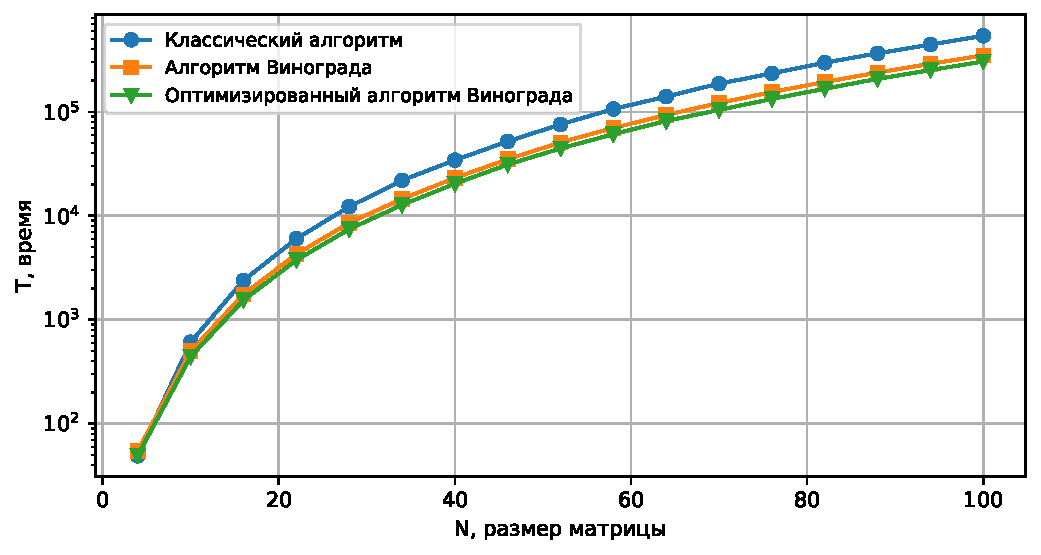
\includegraphics[height=0.3\textheight]{img/graphEven.pdf}
	\caption{Сравнение времени выполнения алгоритмов умножения матриц для четных размеров матриц}
	\label{plt:even_comp_alg}
\end{figure}

Таблица \ref{tbl:odd_time} содержит результаты замеров времени выполнения алгоритмов умножения матриц для нечетных размеров квадратных матриц в диапазоне от 5 до 101 с шагом 6, также с использованием различных входных данных.
\clearpage
\begin{table}[ht]
	\begin{center}
		\begin{threeparttable}
		\small
		\caption{Результаты замеров времени (нечетные размеры матриц)}
		\label{tbl:odd_time}
		\begin{tabular}{|c|c|c|c|}
			\hline
			& \multicolumn{3}{c|}{\bfseries Время, мкс} \\ \cline{2-4}
			\bfseries Размер матрицы & \bfseries Классический & \bfseries Винограда & \bfseries (опт.) Винограда
			\csvreader{csv/dataOdd.csv}{}
			{\\\hline \csvcoli & \csvcolii & \csvcoliii & \csvcoliv} 
			\\
			\hline
		\end{tabular}
		\end{threeparttable}
	\end{center}
\end{table}

На основе данных из таблицы \ref{tbl:odd_time} были построены графики (см. рисунок \ref{plt:odd_comp_alg}), из которых можно сделать вывод, что оптимизированный алгоритм Винограда также является наилучшим выбором для умножения матриц с нечетными размерами.

\begin{figure}[h]
	\centering
	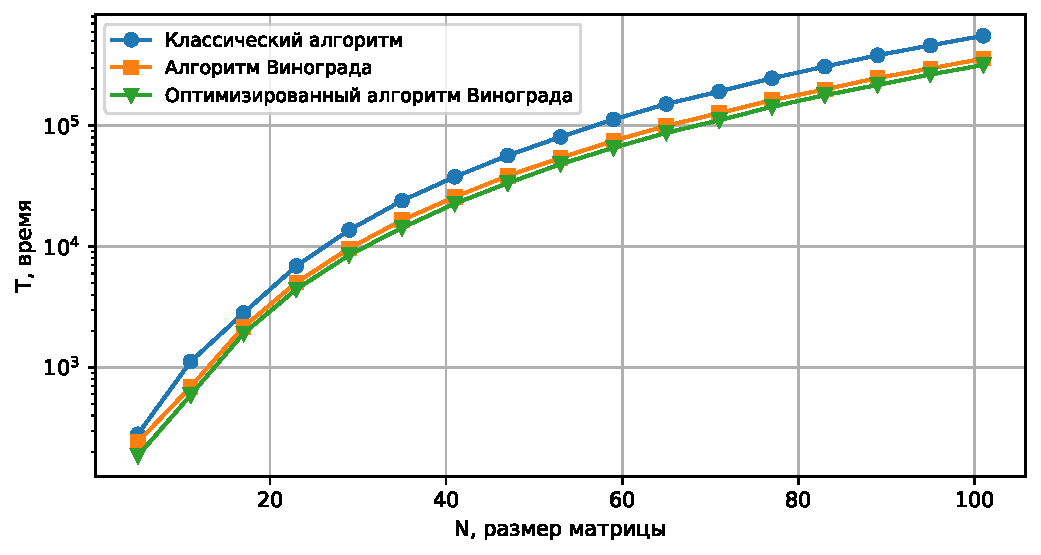
\includegraphics[height=0.3\textheight]{img/graphOdd.pdf}
	\caption{Сравнение времени выполнения алгоритмов умножения матриц для нечетных размеров матриц}
	\label{plt:odd_comp_alg}
\end{figure}
\newpage


\section{Выводы}
Результаты экспериментов позволяют сделать вывод о том, что при больших размерах матриц (более 10), алгоритм Винограда работает значительно быстрее, чем классический алгоритм умножения матриц. 
Оптимизированный алгоритм Винограда в данном контексте демонстрирует лучшие результаты и опережает стандартный алгоритм.

Также было замечено, что алгоритм Винограда на четных размерах матриц работает быстрее по сравнению с нечетными размерами, что объясняется дополнительными вычислениями для крайних строк и столбцов. 
Следовательно, для матриц с четными размерами рекомендуется использовать алгоритм Винограда.